\documentclass[10pt]{article}
\usepackage[top=1in, bottom=1in, left=1in, right=1in]{geometry} % see geometry.pdf on how to lay out the page. There's lots.
\geometry{a4paper}

\usepackage{amsmath}
\usepackage{amssymb}
\usepackage{graphicx}
\usepackage{listings}
\usepackage[usenames,dvipsnames,svgnames,table]{xcolor}

%\usepackage{subcaption}

% comment out if you want automatic paragraph indenting
\setlength{\parindent}{0pt}

\newcommand{\lv}{\lVert}
\newcommand{\rv}{\rVert}
\newcommand{\tl}{\tilde}
\newcommand{\eqn}[1]{
 \begin{align} #1
 \end{align}}

\newcommand*\colvec[3]{
    \begin{pmatrix}#1\\#2\\#3\end{pmatrix}
}

\newcommand*\norm[1]{
  \lVert #1 \rVert
}

\newcommand*\partialDer[2]{
  \frac{\partial #1}{\partial #2}
}


%% To import in the preambule
%\usepackage{listings}

\lstdefinelanguage{ML}{
  alsoletter={*},
  morekeywords={datatype, of, if, *},
  sensitive=true,
  morecomment=[s]{/*}{*/},
  morestring=[b]"
}

% "define" Scala
\lstdefinelanguage{scala}{
  alsoletter={@=>},
  morekeywords={abstract, case, catch, class, def, do, else, extends, false, final, finally, for, if, implicit, import, match, new, null, object,
override, package, private, protected, requires, return, sealed, super, this, throw, trait, try, true, type, val, var, while, with, yield, domain,
postcondition, precondition,invariant, constraint, assert, forAll,  _, return, @generator, ensure, require, ensuring,=>,Real,
certainly, possibly, certify, errorBound, assertBound, jacobian, derivative},%in,
  sensitive=true,
  morecomment=[l]{//},
  morecomment=[s]{/*}{*/},
  showstringspaces=false,
  columns=fullflexible,
  mathescape=true,
  numberstyle=\tiny,
  basicstyle=\codestyle,
  numbersep=5pt,
  stepnumber=2,
  numbers=left,                   % where to put the line-numbers
  morestring=[b]"
}

%\newcommand{\codestyle}{\small\sffamily}
\newcommand{\codestyle}{\small}

\newcommand{\union}{\mbox{\tt ++}}
\newcommand{\difference}{\mbox{\tt --}}
%\newcommand{\RA}{\mbox{\tt =>}}
\newcommand{\RA}{\Rightarrow}
\newcommand{\EQ}{\mbox{\tt ==}}

% Default settings for code listings
\lstset{
%  frame=tb,
  language=scala,
%  aboveskip=3mm,
%  belowskip=3mm,
%  lineskip=-0.1em,
%  numberstyle=\footnotesize,      % the size of the fonts that are used for the line-numbers
%  stepnumber=2,                   % the step between two line-numbers. If it's 1 each line will be numbered
%  numbersep=2pt
}

%\newenvironment{scala}
%        {\lstset{language=scala}\begin{lstlisting}}
%        {\end{lstlisting}}

\newcommand{\pseudostyle}{\sffamily}
% or try smallcaps (yak!)
% \newcommand{\pseudostyle}{\sc}

\lstdefinelanguage{pseudo}{
  alsoletter={@,=,>},
  morekeywords={abstract, case, catch, class, def, do, else, extends, false, final, finally, for, if, implicit, import, match, new, null, object,
override, package, private, protected, requires, return, sealed, super, this, throw, trait, try, true, type, val, var, while, yield, domain, %with
postcondition, invariant, constraint, assert, forAll,  _, return, @generator, ensure, require, ensuring,=>, %precondition
certainly, possibly, certify, errorBound, assertBound, jacobian, derivative, Input, Output},%in,
  sensitive=true,
  morecomment=[l]{//},
  morecomment=[s]{/*}{*/},
  showstringspaces=false,
  columns=fullflexible,
  mathescape=true,
  numberstyle=\tiny,
  basicstyle=\pseudostyle,
  numbers=left,                   % where to put the line-numbers
  morestring=[b]"
}


\newcommand{\lv}{\lVert}
\newcommand{\rv}{\rVert}
\newcommand{\tl}{\tilde}
\newcommand{\eqn}[1]{
 \begin{align} #1
 \end{align}}


\setlength{\parindent}{0pt}



\title{On (More) Precise Propagation of (Roundoff) Errors}
\author{}

\begin{document}

\maketitle

Consider the case of a generic loop, iteratively applying a function $f$.
The following three definitions are equivalent.
\begin{figure}[h!]
  \centering
  \lstset{numbers=none}
  \begin{subfigure}[b]{0.25\textwidth}
    \begin{lstlisting}
var x1 = ???
var x2 = ???
while(i < N) {
  (x1, x2) = f(x1, x2)
}
(x1, x2)
    \end{lstlisting}
  \end{subfigure}%
  \begin{subfigure}[b]{0.32\textwidth}
    \begin{lstlisting}
    val x1, x2 = ???

    def iter(x1, x2, i) = {
      if (i < N) {
        val (y1, y2) = f(x1, x2)
        iter(y1, y2, i + 1)
      } else {
        (x1, x2)
      }
    }
    \end{lstlisting}
  \end{subfigure}
  \begin{subfigure}[b]{0.32\textwidth}
    \begin{lstlisting}
    val x1, x2 = ???

    def iter(x1, x2, i) = {
      if (i < N) {
        val (y1, y2) = iter(x1, x2, i + 1)
        f(y1, y2)
      } else {
        (x1, x2)
      }
    }
    \end{lstlisting}
  \end{subfigure}
\end{figure}


%!TEX root = work-in-progress.tex
\section{}
\label{theory-errors}
We want to find an inductive specification about the output range and output errors.



\paragraph{Notation:} Let
\begin{itemize}
\item $f$ denote the mathematical function $f: \mathbb{R}^n \to \mathbb{R}^n$ or $f: \mathbb{R}^n \to \mathbb{R}$
\item $\tilde{f}$ be the finite-precision version of $f$
\item $\tilde{x}$ be the finite-precision, actually computed, value corresponding to the
ideal variable $x$
\item $\lambda$ be an upper bound on the initial error, i.e. $\lv x - \tilde{x} \rv$
\item $\sigma$ be the roundoff error on evaluating $f$ with exact inputs, i.e.
  $\lv f(x) - \tilde{f}(x) \rv$
\end{itemize}
where $f$ and $x$ may be vectors, in which case the definitions are component-wise.

\subsection{Division of error}
The overall error on evaluating $f: \mathbb{R}^n \to \mathbb{R}$ in finite-precision arithmetic is
  $\lv f(x) - \tilde{f}(\tilde{x}) \rv$, where $\lv x - \tilde{x} \rv \le \lambda$.

\begin{align}
\lv f(x) - \tilde{f}(\tilde{x}) \rv &=
 \lv f(x) - f(\tilde{x}) + f(\tilde{x}) - \tilde{f}(\tilde{x}) \rv \\
 &\le \lv f(x) - f(\tilde{x}) \rv + \lv f(\tilde{x}) - \tilde{f}(\tilde{x}) \rv
\end{align}

Suppose there is a function $g: \mathbb{R} \to \mathbb{R}$, such that $\lv f(x) - f(y) \rv \le g(\lv x - y \rv)$.
Further note that $\lv f(\tilde{x}) - \tilde{f}(\tilde{x}) \rv$ is the roundoff error on
computing $f$ with exact inputs. Then,

\begin{align}
\label{errorLoopBody}
\lv f(x) - \tilde{f}(\tilde{x}) \rv &\le g(\lv x - \tilde{x} \rv) + \sigma
\end{align}
We have thus separated the overall error into the error from propagating
the initial uncertainty and the roundoff error.

Consider iterating $f$, i.e. we are computing $f^n(x) = f(f(...f(x)))$.

{\bf Claim: }
\begin{equation}
\lv f^n(x) - \tl{f}^n(\tl{x})\rv \le \sigma + \sum^{n - 1}_{i = 1} g^i(\sigma) + g^n(\lv x - \tl{x} \rv)
\end{equation}

We show this by induction. The base case, for $n = 1$ is shown above.
\begin{align}
\lv  f^n(x) - \tl{f}^n(\tl{x})\rv &\le
  \lv f^n(x) - f(\tl{f}^{n-1}(\tl{x})) \rv + \lv f(\tl{f}^{n-1}(\tl{x})) - \tl{f}^n(\tl{x})\rv \\
  &\le g(\lv f^{n-1}(x) - \tl{f}^{n-1}(\tl{x}) \rv) + \sigma \\
  &\le g (\sigma + \sum^{n - 2}_{i = 1} g^i(\sigma) + g^{n-1}(\lv x - \tl{x} \rv)) + \sigma \\
  &\le \sigma + \sum^{n - 1}_{i = 1} g^i(\sigma) + g^n(\lv x - \tl{x} \rv)
\end{align}


\subsection{Multivariate case}
In the above computation, we compute the error for each component separately, i.e. $f: \mathbb{R}^n \to \mathbb{R}$.
Since $g: \mathbb{R} \to \mathbb{R}$ and we are computing $g(\lv x - \tilde{x} \rv$, we are loosing
precision since we do not consider the error contributions from different inputs separately.
For instance, when using the infinity norm, we only consider the largest error.

Now suppose $f, g: \mathbb{R}^n \to \mathbb{R}^n$ and $x, \tilde{x}, \sigma, \lambda \in \mathbb{R}^n$.

We want to compute the error on every component of $f$, i.e. $\lv f_i(x) - \tilde{f}_i(\tilde{x}) \rv$,
where $\lv x_i - \tilde{x}_i \rv \le \lambda_i$, for $i \in 1 \dots n$.


\begin{align}
\lv f_i(x) - \tilde{f}_i(\tilde{x}) \rv &=
 \lv f_i(x) - f_i(\tilde{x}) + f_i(\tilde{x}) - \tilde{f}_i(\tilde{x}) \rv \\
 &\le \lv f_i(x) - f_i(\tilde{x}) \rv + \lv f_i(\tilde{x}) - \tilde{f}_i(\tilde{x}) \rv
\end{align}

$g: \mathbb{R}^n \to \mathbb{R}^n$, such that
$\lv f_i(x) - f_i(y) \rv \le g_i(\lv x_1 - y_1\rv, ..., \lv x_n - y_n\rv)$
and $\sigma_i = \lv f_i(\tilde{x}) - \tilde{f}_i(\tilde{x}) \rv$, the roundoff error on
computing $f$ with exact inputs. Then,

\eqn{
\label{errorLoopBodyMulti}
\norm{ f_i(x) - \tilde{f}_i(\tilde{x})} &\le g_i(\norm{ x_1 - y_1}, ..., \norm{ x_n - y_n }) + \sigma_i\\
&= g_i(\vec{\lambda}) + \sigma_i
}


Consider iterating $f$, i.e. we are computing $f^n(x) = f(f(...f(x)))$.

{\bf Claim: }
\eqn{
\norm{ f^m(x)_i - \tl{f}^m(\tl{x})_i } \le \left( \sigma + \sum^{m - 1}_{j = 1} g^j(\sigma) + g^m(\norm{x - \tl{x}}) \right)_i
}

We show this by induction. The base case, for $n = 1$ is shown above.
\eqn{
  \colvec{\norm{f^m(x)_1 - \tl{f}^m(\tl{x})_1}}{\vdots}{\norm{f^m(x)_n - \tl{f}^m(\tl{x})_n}} &\le
  \colvec{
  \norm{f^m(x)_1 - f(\tl{f}^{m-1}(\tl{x}))_1} + \norm{f(\tl{f}^{m-1}(\tl{x}))_1 -\tl{f}^m(\tl{x}_1) }
  }{\vdots}{
  \norm{f^m(x)_n - f(\tl{f}^{m-1}(\tl{x}))_n} + \norm{f(\tl{f}^{m-1}(\tl{x}))_n -\tl{f}^m(\tl{x}_n) }}\\
  &\le g\colvec{
  \norm{f^m(x)_1 - f(\tl{f}^{m-1}(\tl{x}))_1}}{\vdots}{\norm{f^m(x)_n - f(\tl{f}^{m-1}(\tl{x}))_n}} +
  \colvec{\sigma_1}{\vdots}{\sigma_n}\\
  &\le g \left(\vec{\sigma} + \sum^{m-2}_{j = 1} g^j(\vec{\sigma}) + g^{m-1}(\vec{\lambda}) \right)+ \vec{\sigma}\\
  &=\sum^{m-1}_{j = 1} g^j(\vec{\sigma}) + g^m(\vec{\lambda}) + \vec{\sigma}
}



\subsection{Lipschitz continuity}
Now consider $g(x) = K \cdot x$, i.e. which yields Lipschitz continuity:
$\lv f(x) - f(y) \rv \le K \lv x - y \rv$.
Note that we need to compute the Lipschitz constant for the mathematical function $f$,
and not for $\tl{f}$.
The expression for the error then becomes
\begin{align}
\lv f^n(x) - \tl{f}^n(\tl{x})\rv \le K^n \lambda + \sum^{n-1}_{i=0}K^i \sigma
  = K^n \lambda + \sigma \sum^{n-1}_{i=0} K^i
  = K^n \lambda + \sigma \left(\dfrac{1 - K^n}{1-K} \right)
\end{align}
when $K \ne 1$.
When $K = 1$, $g$ becomes the identity function and so
\begin{align}
\lv f^n(x) - \tl{f}^n(\tl{x})\rv \le \sigma + \sum^{n-1}_{i=1}\sigma + \lambda
= n \cdot \sigma + \lambda
\end{align}

We want to compute the Lipschitz constant for a function $f: \mathbb{R}^n \to \mathbb{R}$,
that is, we are computing one constant for each output of the function.

Let $h: [0, 1] \to \mathbb{R}$ such that $h(\theta) := f(z + \theta(y-z))$.
Then $h(0) = f(z)$ and $h(1) = f(y)$ and
\eqn{
  \frac{d}{d\theta}h(\theta) &= \nabla f(z + \theta(y-z)) \cdot (y-z)
}

By the mean value theorem:
\eqn{
  f(y) - f(z) &= h(1) - h(0) = h'(\zeta) \qquad \text{ where } \eta \in [0, 1] \\
}

\eqn{
   \lv f(y) - f(z) \rv &= \lv h'(\zeta) \rv\\
&\le\lv \nabla f(z + \zeta(y-z)) \cdot (y-z) \rv \\
&\le \sup\limits_{\theta\in [0,1]} \lv \nabla f(z + \theta(y-z))  \cdot (y-z) \rv\\
&\le \sup\limits_{\theta\in [0,1]} \lv \nabla f(z + \theta(y-z))  \rv \rv (y-z) \rv
}

% \eqn{
%   f(y) - f(z) &= h(1) - h(0) = \int^1_0 h'(\theta)d\theta
%   = \int^1_0\nabla f(z + \theta(y-z)) d\theta \cdot (y-z)
% }

% \eqn{
%   \lv f(y) - f(z) \rv &= \lv \int^1_0\nabla f(z + \theta(y-z)) d\theta \cdot (y-z) \rv \\
% &le \int^1_0 \lv \nabla f(z + \theta(y-z))  \cdot (y-z) \rv d\theta \quad
%    \text{ (triangle inequality for integrals)}\\
% &\le \sup\limits_{\theta\in [0,1]} \lv \nabla f(z + \theta(y-z))  \cdot (y-z) \rv \int^1_0 d\theta\\
% \label{eqnG}
% &= \sup\limits_{\theta\in [0,1]} \lv \nabla f(z + \theta(y-z))  \cdot (y-z) \rv \\
% &\le \sup\limits_{\theta\in [0,1]} \lv \nabla f(z + \theta(y-z))  \rv \rv (y-z) \rv
% }

Since $f(y) - f(z) \in \mathbb{R}$, all vectors norms $\lv f(y) - f(z) \rv$
are equivalent to $|f(y) - f(z)|$ and we can choose any norm.

% If possible (and correct!), for precision reasons, we may want to already use Equation \ref{eqnG}  i.e.
% \eqn{
%   g(x) = \sup\limits_{\theta\in [0,1]} \lv \nabla f(z + \theta(y-z))(x)\rv
% }

Thus, in order to compute the Lipschitz constant, we need to bound the gradient of $f$
over the specified input range.



\subsubsection{Multivariate case}
Let $h: [0, 1] \to \mathbb{R}^n$ such that $h(\theta) := f(z + \theta(y-z))$.
Then $h(0) = f(z)$ and $h(1) = f(y)$ and
\eqn{
  \frac{d}{d\theta}h(\theta) &= \nabla f(z + \theta(y-z)) \cdot (y-z)
}

By the mean value theorem:
\eqn{
  f(y) - f(z) &= h(1) - h(0) = h'(\zeta) \qquad \text{ where } \eta \in [0, 1] \\
}
\eqn{
   \norm{ f_i(y) - f_i(z) } &= \norm{ h_i'(\zeta) }\\
&\le \norm{ \left( \nabla f(z + \zeta(y-z)) \cdot (y-z) \right)_i } \\
&= \norm{ \left(
\begin{pmatrix}
\partialDer{f_1}{w_1} & \dots & \partialDer{f_1}{w_n}\\
\dots \\
\partialDer{f_n}{w_1} & \dots & \partialDer{f_n}{w_n}
\end{pmatrix}\cdot (y-z) \right)_i }\\
&= \norm{
\partialDer{f_i}{w_1} \cdot (y_1 - z_1) + \dots + \partialDer{f_i}{w_n} \cdot (y_n - z_n)}\\
%&\le \sup\limits_{\theta\in [0,1]} \lv \nabla f(z + \theta(y-z))  \cdot (y-z) \rv\\
%&\le \sup\limits_{\theta\in [0,1]} \lv \nabla f(z + \theta(y-z))  \rv \rv (y-z) \rv
}

Hence, we get
\begin{align}
\lv f^n(x) - \tl{f}^n(\tl{x})\rv &\le K^n \lambda + \sum^{n-1}_{i=0}K^i \sigma\\
  &= K^n \lambda + (\sum^{n-1}_{i=0} K^i) \sigma\\
  &= K^n \lambda + ( (I-K)^{-1}(I - K^n) )\sigma
\end{align}
where $K$ is now a matrix with $K_{ij} = sup(\partialDer{f_i}{w_j})$.

\subsection{A little bit of linear algebra}
For the multivariate case, we need to evaluate $K^n$ and $(I-K)^{-1}(I - K^n)$,
where $K$ is a matrix. There are two options:
\begin{enumerate}
\item Do the actual iteration. We use rationals, hence the result is going to be accurate,
and thus sound, although not efficient for large $n$. Also, for dimensions up to 3,
computing the inverse can be done with an analytic expression. For larger dimensions,
this approach becomes impractical.

\item Find a basis transform $P$ such that we can bring $K$ into Jordan normal form.
That is, we want to find $P, D$ such that $K = P^{-1}DP$ where $D$ is block diagonal.
The big question is, how do you find the basis transformation and how do you compute the
eigenvalues/$D$.
\end{enumerate}




%\subsection{Applications}
%\begin{itemize}
%\item more precise error computation
%\item loops
%\item modular composition of functions
%\item input sensitivity information
%\end{itemize}


\section{Preliminary manual experiments}

\subsection{Harmonic oscillator}
\eqn{
  f_1(x, v) &= x + v \cdot dt\\
  f_2(x, v) &= v - k \cdot x \cdot dt
}

Assume input ranges $x \in [0.15, 0.25]$ and $v \in [3.35, 3.45]$
and parameter $k = 2.3, dt = 0.1$.
Then $K = 1$ and our method can recover that errors are merely being added in this case.


\begin{figure}[h!]
  \centering
\begin{subfigure}[b]{0.45\textwidth}
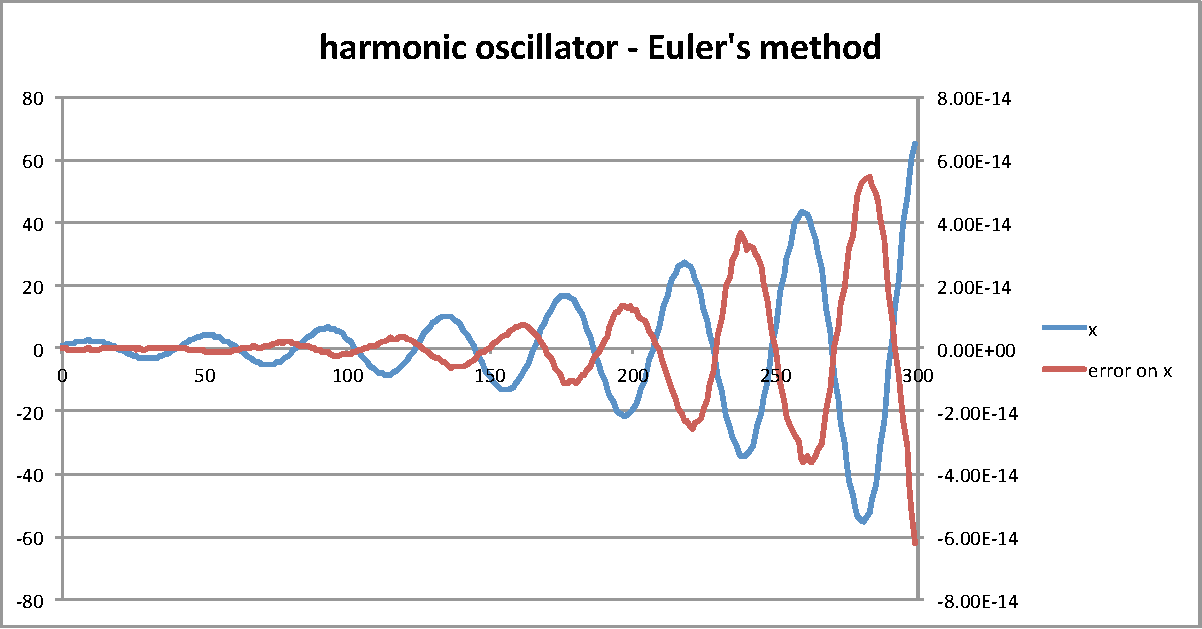
\includegraphics[width=\textwidth]{images/harmonic_euler}
%\caption{A gull}
%\label{fig:gull}
\end{subfigure}%
~ %add desired spacing between images, e. g. ~, \quad, \qquad etc.
  %(or a blank line to force the subfigure onto a new line)
\begin{subfigure}[b]{0.45\textwidth}
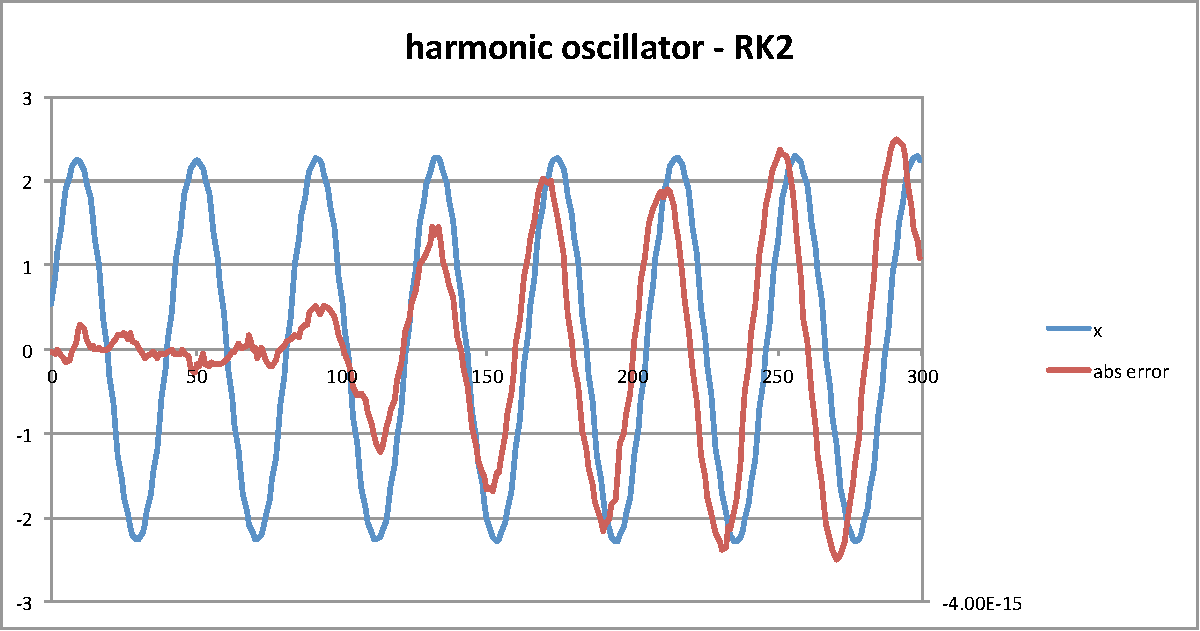
\includegraphics[width=\textwidth]{images/harmonic_rk2}
%\caption{A tiger}
%\label{fig:tiger}
\end{subfigure}
\caption{True errors for harmonic oscillator}
\label{fig:harmonic}
\end{figure}




\subsection{2-body simulation}
\begin{figure}[h!]
  \centering
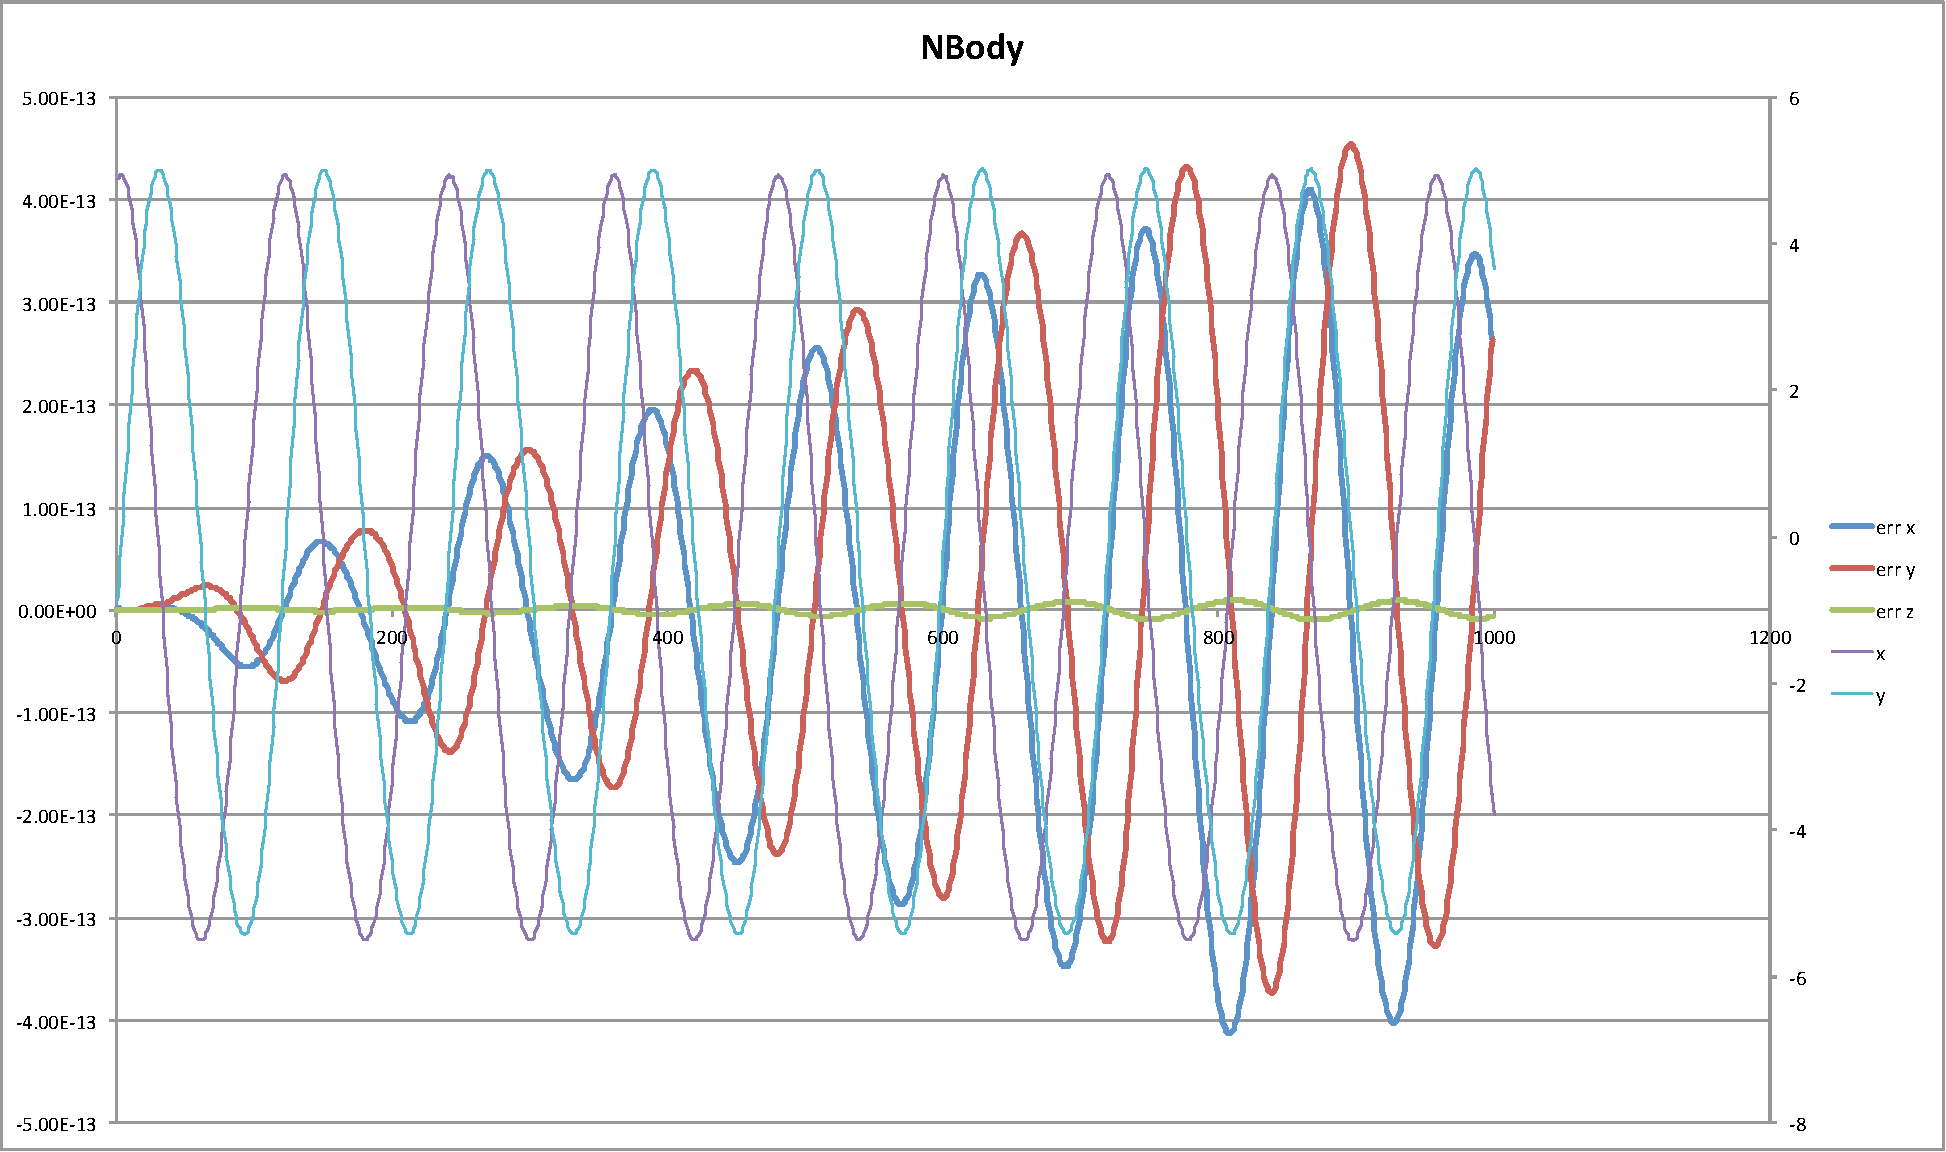
\includegraphics[width=\textwidth]{images/nbody}
  \caption{True errors for nbody simulation}
\label{fig:2body}
\end{figure}

\subsection{Predator-Prey}
Simulation of a hare and lynx population.
\eqn{
  \frac{dH}{dt} &= r H (1 - \frac{H}{k}) - \frac{a H L}{c + H}\\
  \frac{dL}{dt} &= \frac{b a H L}{c + H} - d L
}
$a = 3.2, b = 0.6, c = 50, d = 0.56, k = 125.0, r = 1.6$
$H \in [0, 90], L \in [0, 90]$

Solving this with Euler's method:
\eqn{
  f_1 = H + dt * \frac{dH}{dt} \qquad f_2 = L + dt * \frac{dL}{dt}
}

We have (so far) computed
\eqn{
  \sup \frac{\partial f_1}{\partial H} \le 1.6
}
This is bad news, since it means that after only 10 iterations, roundoff errors
get magnified by a factor of 182 (as computed with $\frac{1-K^n}{1-K}$).

A quick experiment showed, however, that if can constraint the variables further,
for example by using some (hopefully present) relationship between $H$ and $L$,
then we can also shrink the Lipschitz constant $K$.


\begin{figure}[h!]
  \centering
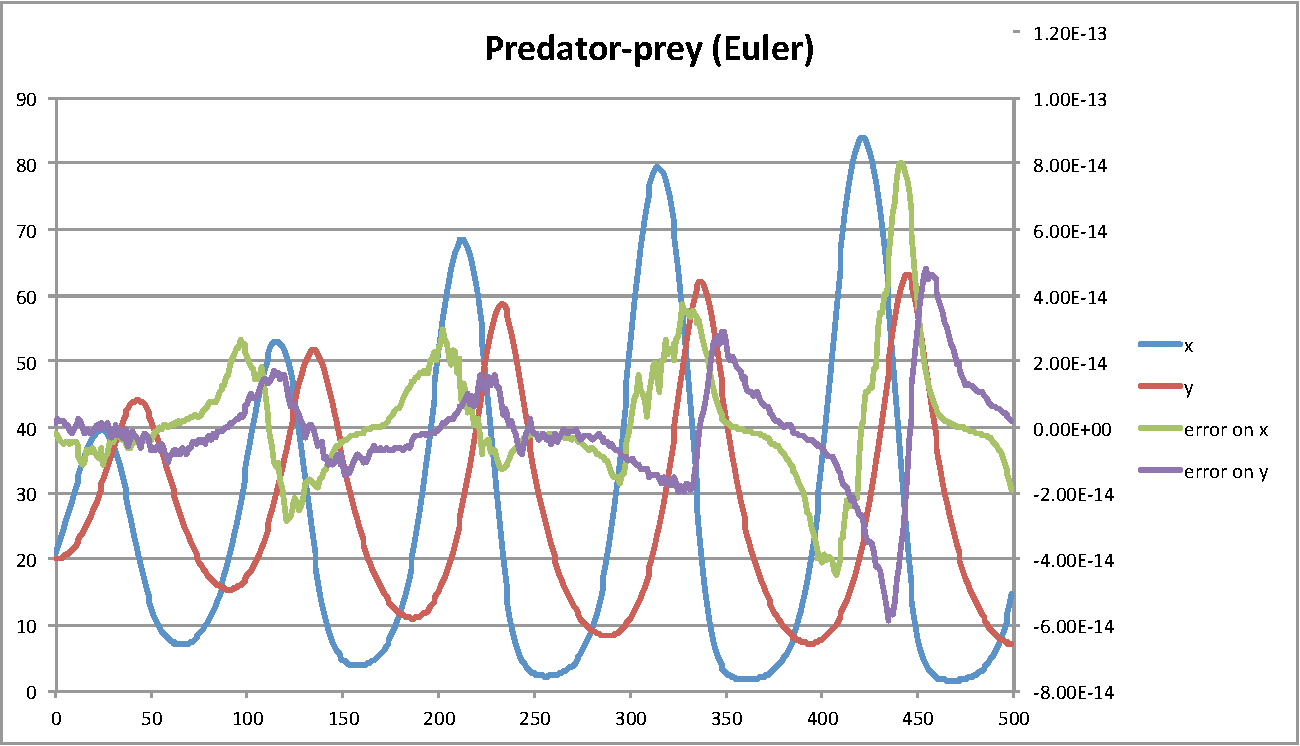
\includegraphics[width=\textwidth]{images/predator-prey}
  \caption{True errors for predator-prey simulation}
\label{fig:predator}
\end{figure}

\subsection{Jet engine and doppler revisited}
We can use Equation~\ref{errorLoopBody} to compute the overall error for
a loop-free function.
The jet-engine example is function of two variables $f(x_1, x_2)$.
Using our range computation we can bound the components of the gradient
over the input ranges $x_1 \in [-5, 5], x_2 \in [-20, 5]$
\eqn{
  \frac{d f}{d x_1} \in [-3555, 3440] \qquad \frac{d f}{d x_2} \in [-152, 270]
}
The roundoff error for exact inputs is $1.61703982148642E-08$, as computed by Rosa.
Then, including the initial errors on $x_1, x_2 = 1e-8$, we have by
Equation~\ref{errorLoopBody}:
\eqn{
\text{total error} \le \sigma + K * \lambda \le 1.62e-08 + 3555 * 1e-8 = 3.557e-8
}
The total error computed for this example computed by Rosa with our old technique
is $0.140017339985495$, four orders of magnitude larger.

Similarly, for the computation of the doppler shift (a much smaller, but nonlinear example),
we can approximately half the error from $2.35478453236889e-06$ to $1.13e-6$.

\subsection{Further experiments:}
Mean, standard deviation and variance, damped oscillator.
To follow.

%\subsection{Newton's method}

% \section{Possible extensions}
% \subsection{Adding other errors within the same model}
% e.g. truncation errors, as long as they only depend on the range in some way

% \section{Other aspects}

% specification language allowing different inductive formulations
\end{document}
